\graphicspath{{Introduction/figures/}}
\chapter{Introduction}\label{ch:intro}
%\thispagestyle{empty}

\runningchaptertitle{Introduction}
%\bstctlcite{IEEE:BSTcontrol}
%% Use this code to put your background image
%\ThisCenterWallPaper{\wpScaling}{ChapterBackground.png}
%\noabstract
\ThumbIndexShow

\newcommand{\tb}{\textit{{\textbf{}}}}



\section{Pulmonary anatomy}


\section{Systemic sclerosis}
Systemic sclerosis (SSc) is an immune-mediated rheumatic disease that is characterised by fibrosis of the skin and internal organs and vasculopathy \cite{denton2017systemic}. Although systemic sclerosis is uncommon, it has a high morbidity — greater than any other rheumatic disease \cite{denton2017systemic}. Lung fibrosis or interstitial lung disease (ILD) is the primary contribuor of death, followed by Pulmonary arterial hypertension (PAH) and cardiac causes  \cite{Acharya2013, steele2012clinical}. ILD is present in 80\% of patients with systemic sclerosis \cite{codes2023systemic}. The main tools to diagnosis SSc related ILD (SSc-ILD) include pulmonary function tests and chest CT scans \cite{codes2023systemic}.

\section{Pulmonary function tests}

To evaluate progression of SSc-ILD, various pulmonary function tests (PFTs) are used as key measures \cite{Behr2008, Caron2018, Ninaber2015}, such as the diffusion capacity for carbon monoxide (DLCO), forced expiratory volume in 1 second (FEV\textsubscript{1}), forced vital capacity (FVC) and total lung capacity (TLC). 

\begin{itemize} 
\item DLCO. DLCO is a measurement to assess the lungs' ability to transfer gas from inspired air to the bloodstream \cite{Graham2017} (see Figure \ref{fig:chap1_dlco}). Carbon monoxide (CO) is used for this test because it has a higher affinity for hemoglobin (200 to 250 times that of oxygen), and it follows the same pathway as that of oxygen to finally bind with hemoglobin. Oxygen is not preferred since its uptake is limited by cardiac uptake and total body consumption \cite{mehra2017evaluation}. DLCO is expressed as mL/min/mm Hg, represents mL of CO transferred per minute for each mm Hg of pressure difference across the total available functioning lung gas exchange surface \cite{macintyre2005standardisation}. 

\item FEV\textsubscript{1}. FEV\textsubscript{1} is the amount of air exhaled during the first second of the FVC maneuver (Figure \ref{fig:chap1_pft}). It tends to be lower in diseases that obstruct the airway, such as asthma or emphysema.

\item FVC. A breathing curve begins with the patient inhaling as deeply as he or she can. Then the patient exhales as long and as forcefully as possible; the amount exhaled in this manner is the FVC (Figure \ref{fig:chap1_pft}).

\item TLC. Even after one exhales as long and as hard as possible, some air remains in the lungs; this is called the residual volume (RV). The residual volume plus the FVC equals the TLC (see Figure \ref{fig:chap1_pft}). The RV (and hence the TLC) cannot be measured by spirometry. Rather, they must be measured by special tests that require the patient either to breathe an inert gas such as helium (the concentration of which is measured in the expired air, from which the residual volume is calculated) or to sit in an airtight booth in which the pressure is measured as he or she breathes. 

\end{itemize}



\begin{figure}[tb]
    \centering
    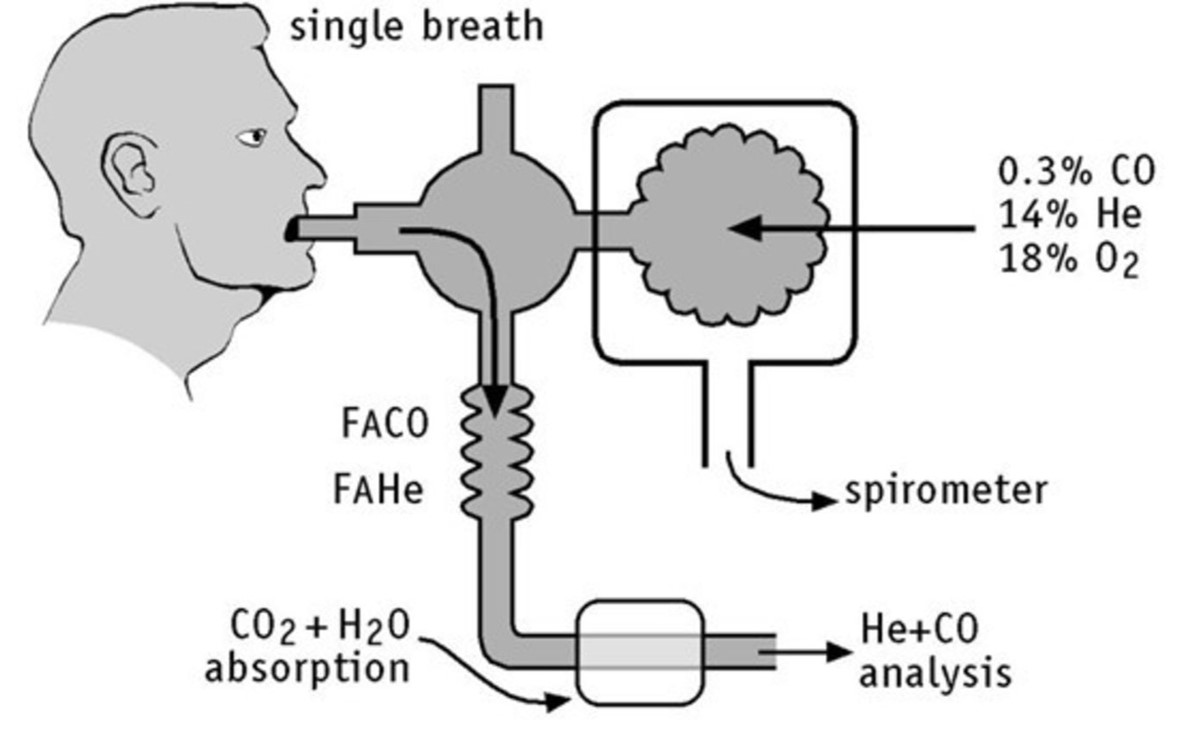
\includegraphics[width=0.6\textwidth]{Introduction/figures/dlco.jpg}
    \caption{Illustration of DLCO measurement. FACO: Fraction of Carbon Monoxide in Alveolar Gas. FAHE: Fraction of Helium in Alveolar Gas. (adopted from \cite{Sylvester2020}).}
    \label{fig:chap1_dlco}
\end{figure}




\begin{figure}[tb]
    \centering
    
\includegraphics[width=0.8\textwidth]{Introduction/figures/PFTs.png}
    \caption{Breathing curve measured by spirometry. RV: residual volume, FEV\textsubscript{1}: forced expiratory volume in 1 second, FVC: forced vital capacity, TLC: total lung capacity (adopted and modified from \url{https://bronchiectasis.com.au/bronchiectasis/diagnosis-2/lung-function}).}
    \label{fig:chap1_pft}
\end{figure}



PFTs can, however, not always be performed if there is a risk of disease transmission, e.g. in patients with COVID-19, active tuberculosis or other airborne infectious diseases \cite{choi2022automated, McGowan2022}. In addition, some patients, who have hemoptysis or had surgery in the past month, or other contraindications \cite{Cooper, Meng2023}, like aneurysmatic abnormalities and ischaemic stroke, are not able to perform PFTs because the forced exhalation during spirometry may increase the risk of complications [9].

\section{Chest CT}
According to expert consensus, PFTs should be ordered in all patients with SSc and repeated regularly to monitor the progress of SSc \cite{hoffmann2020identification}. However, some patients with SSc, particularly those with anti-topoisomerase antibodies, have normal FVC and DLCO values despite the presence of fibrosis on computed tomography (CT) \cite{showalter2018performance}. Therefore, CT also plays an import role on the accurate diagnosis of SSc.

CT, as a non-invasive imaging technique, is the gold standard for the detection of ILD in SSc disease \cite{codes2023systemic}. A chest CT scan offers a more intricate visualization compared to a standard chest X-ray. It captures multiple views of the lungs, which are then combined into three-dimensional, cross-sectional representations, visualizing the organs' dimensions, contours, and internal architecture. CT could provide valuable findings including the pattern of ILD (e.g. ground glass opacity and reticulation shown in Figure \ref{fig:chap1_ct_samples}) and the severity or extent of fibrosis, findings that correlate with disease prognosis \cite{silver2015management}. Expert consensus guidelines recommend that CT should be performed in all SSc patients to screen for ILD \cite{hoffmann2020identification}.

\begin{figure}[tb]
    \centering
    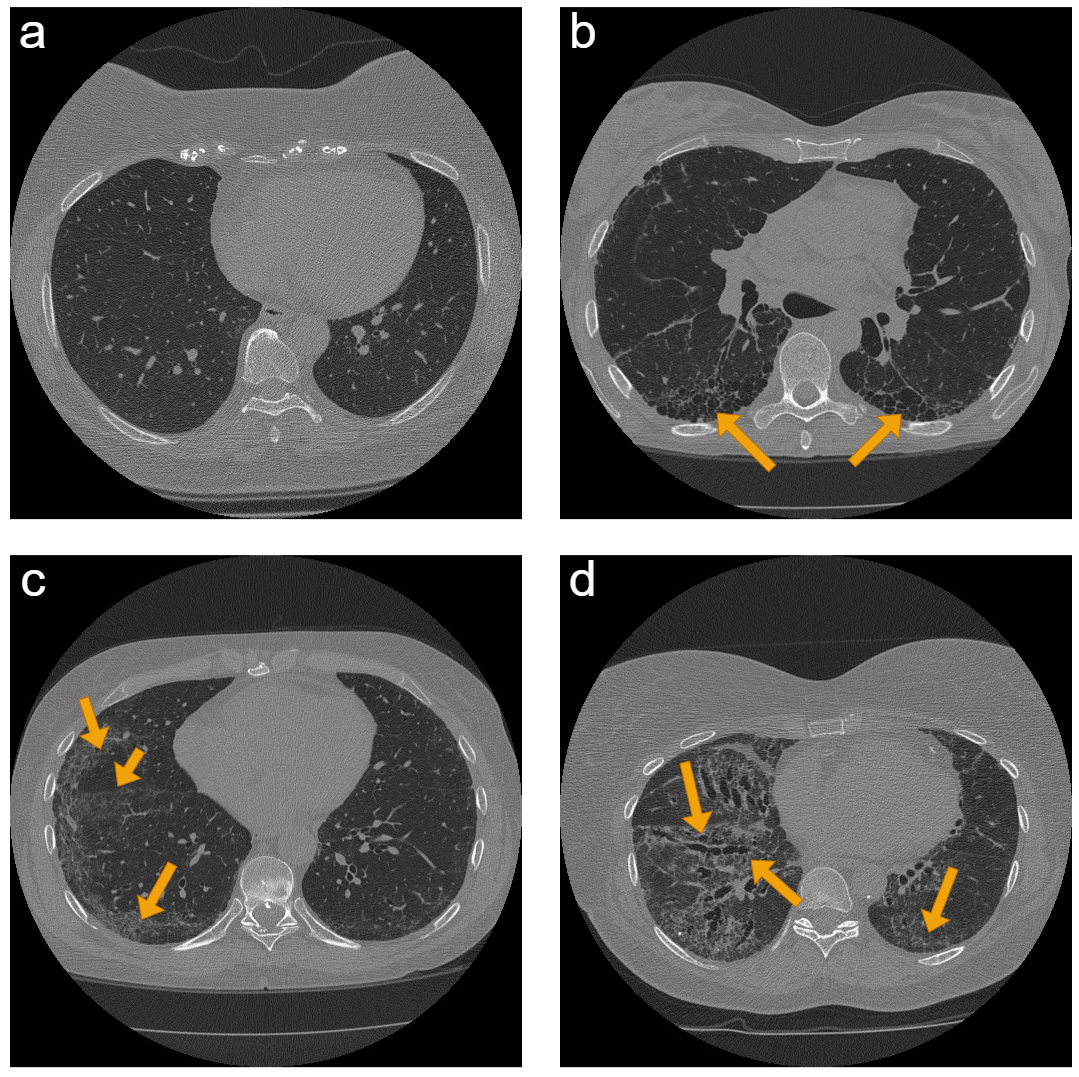
\includegraphics[width=0.8\textwidth]{Introduction/figures/ct_samples.png}
    \caption{Slices of CT scans from a SSc patient with different patterns (arrows). a) normal case, b) with reticulation pattern, c) with ground glass opacity pattern, d) with reticulation and ground glass opacity pattern pattern.}
    \label{fig:chap1_ct_samples}
\end{figure}



\section{Deep learning on chest CT understanding}
Although CT could provide detailed information and Several scoring systems have been proposed to quantify SSc-ILD from chest CT scans, it is still a challenging task to diagnosize SSc disease. Because 1) visual scoring is subjective and significantly rely on the exprience of clinicians. Especially when recognizing different patterns and estimating their area. 2) a high-resolution CT normally include more than 500 slices, which significantly increase the diagnostic workload for clinicians. In addition, 

because of difficulties in  to the whole lung. ILD scoring is still laborious and dependent on rater experience. 

Therefore, an automatic scoring tool is important for a objective, efficient and accurate diagnosis. In addition, we can also explore more biomarkers based on automatic tools.


\section{Thesis outline}

The aim of this thesis is to develop these methods focusing on quantifying disease sevirity of SSc disease based on CT images. The research topics and connections between each chapter are summarized in Figure *. 


%\begin{description}[align=left]
\textbf{Chapter 2} developed a deep learning based network for lobe segmentation. We proposed a multi-task semi-supervised model that can leverage information of multiple structures from unannotated datasets and datasets annotated with different structures. A focused alternating training strategy is presented to balance the different tasks. We evaluated the trained model on an external independent CT dataset. The results show that our model significantly outperforms single-task alternatives. We also demonstrated that our approach is successful for different network architectures as backbones. 

\textbf{ Chapter 3} 

\textbf{Chapter 4} proposed a deep learning based framework to automatically estimate PFT results from chest CT scans of SSc patients. We use segmented lungs and vessels to mask the CT images seperately to explore how different regions influence the estimation of PFTs. We also proposed regression attention maps (RAM), which showed the contribution of different regions. This suggests that that manually designed imaging biomarkers can still contribute to explaining the relation between lung function and structure.

\textbf{Chapter 5} 

\textbf{Chapter 6} summarizes and discusses the overall achievements of this thesis.

%\end{description}
